\documentclass{article}

\usepackage[margin=1in]{geometry}
\usepackage{amssymb, amssymb, amsthm}
\usepackage{enumitem}
\usepackage{courier}
\usepackage{listings}
\usepackage{graphicx}
\usepackage{fancyvrb}
\usepackage{color}
\usepackage{hyperref}

\definecolor{bgcolor}{rgb}{0.9, 0.9, 0.9}
\definecolor{light}{rgb}{0.5, 0.5, 0.5}
\def\light#1{{\color{light}#1}}

\lstset
{
    language=Python,
    numbers=left,
    stepnumber=1,
    showstringspaces=false,
    tabsize=4,
    breaklines=true,
    breakatwhitespace=false,
}

\begin{document}
\pagenumbering{gobble}

\begin{flushright}
Keegan Dahm \\
W207 \\
Lab 1
\end{flushright}

All my source files are at \href{https://github.com/TehVulpes/W207-Lab-1}{https://github.com/TehVulpes/W207-Lab-1}.

\begin{enumerate}[start=1]
\item % 1
    ~\\
    \begin{center}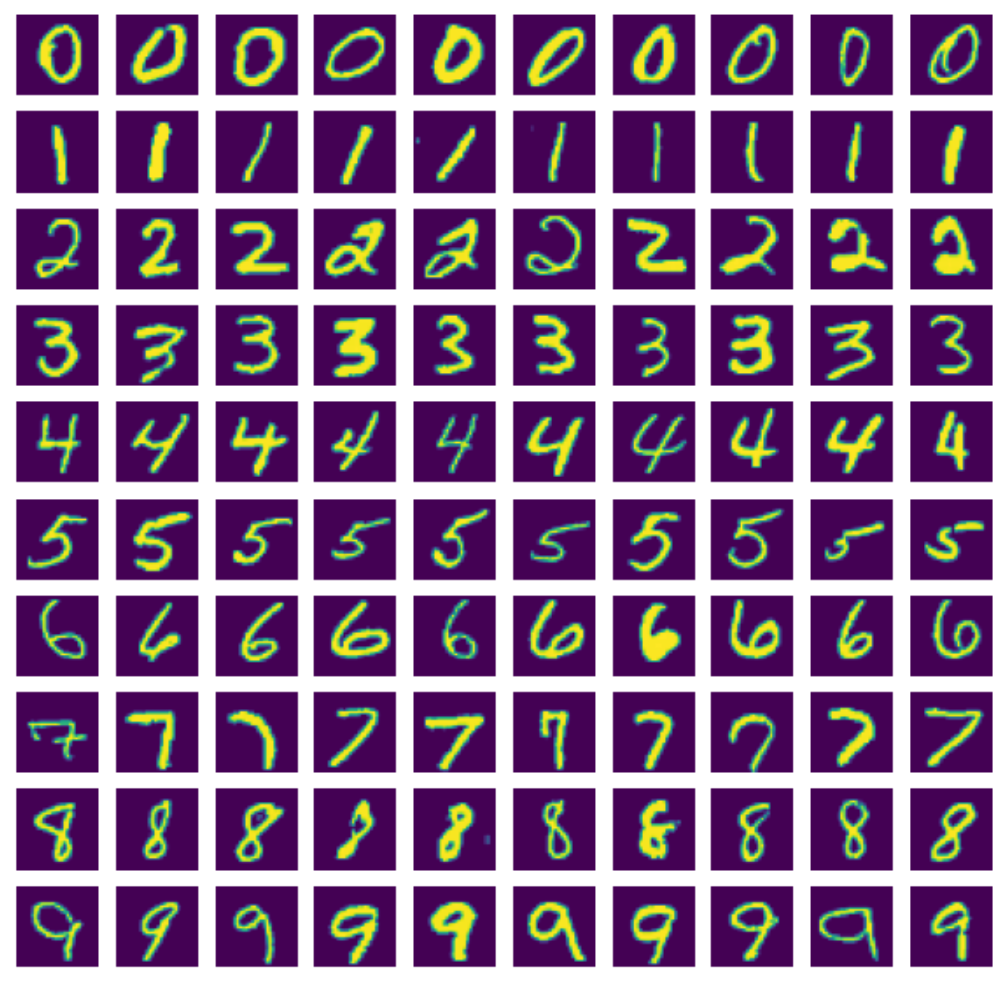
\includegraphics[width=8cm]{1.png}\end{center}

\item % 2
    For K nearest neighbors, with K = 1, the classifier had the hardest time recognizing '9'.
    
    The output of my section 2, with accuracy, is as below:
    
    \begin{Verbatim}[commandchars=+\[\]]
k: 1
              precision    recall  f1-score   support

           0       0.95      0.95      0.95       106
           1       0.89      0.98      0.93       118
           2       0.90      0.79      0.84       106
           3       0.93      0.87      0.90        97
           4       0.91      0.85      0.88        92
           5       0.86      0.88      0.87        88
           6       0.92      0.92      0.92       102
           7       0.85      0.94      0.89       102
           8       0.83      0.77      0.80        94
           9       0.80      0.86      0.83        95

    accuracy                           0.88      1000
   macro avg       0.88      0.88      0.88      1000
weighted avg       0.89      0.88      0.88      1000

k: 3	accuracy: 0.876
k: 5	accuracy: 0.882
k: 7	accuracy: 0.877
k: 9	accuracy: 0.875
    \end{Verbatim}
    
\newpage

\item % 3
    The following table shows the accuracy and evaluation time of each Nearest Neighbors classifier.
    
    \begin{tabular}{| c | c | c |}
    \hline
    \textbf{No. Data Points} & \textbf{Accuracy} & \textbf{Evaluation Time (seconds)} \\
    \hline
    100 & 0.70 & 0.175 \\
    \hline
    200 & 0.79 & 0.341 \\
    \hline
    400 & 0.81 & 0.652 \\
    \hline
    800 & 0.87 & 1.326 \\
    \hline
    1,600 & 0.91 & 2.654 \\
    \hline
    3,200 & 0.93 & 5.388 \\
    \hline
    6,400 & 0.94 & 10.804 \\
    \hline
    12,800 & 0.95 & 21.600 \\
    \hline
    25,600 & 0.96 & 43.238 \\
    \hline
    \end{tabular}
    
    As this table shows, classification time increases linearly with the training size, while accuracy plateaus.
    
\item % 4
    The following graphs show the accuracy of the Nearest Neighbor Classifier and the predicted accuracy using a linear regression model (left), and the accuracy predicted from the log of the training size (right).
    
    \begin{center}
    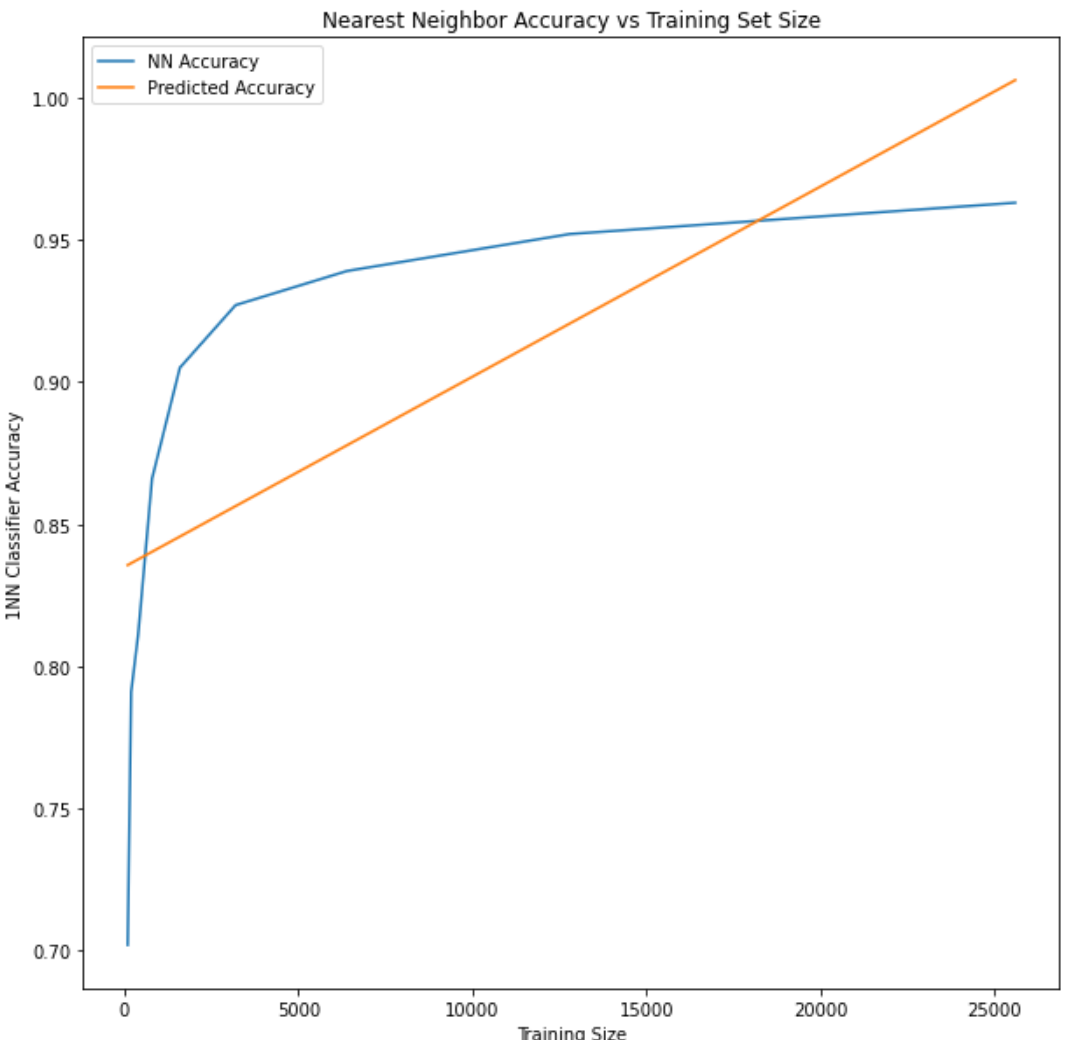
\includegraphics[width=7cm]{4.1.png}
    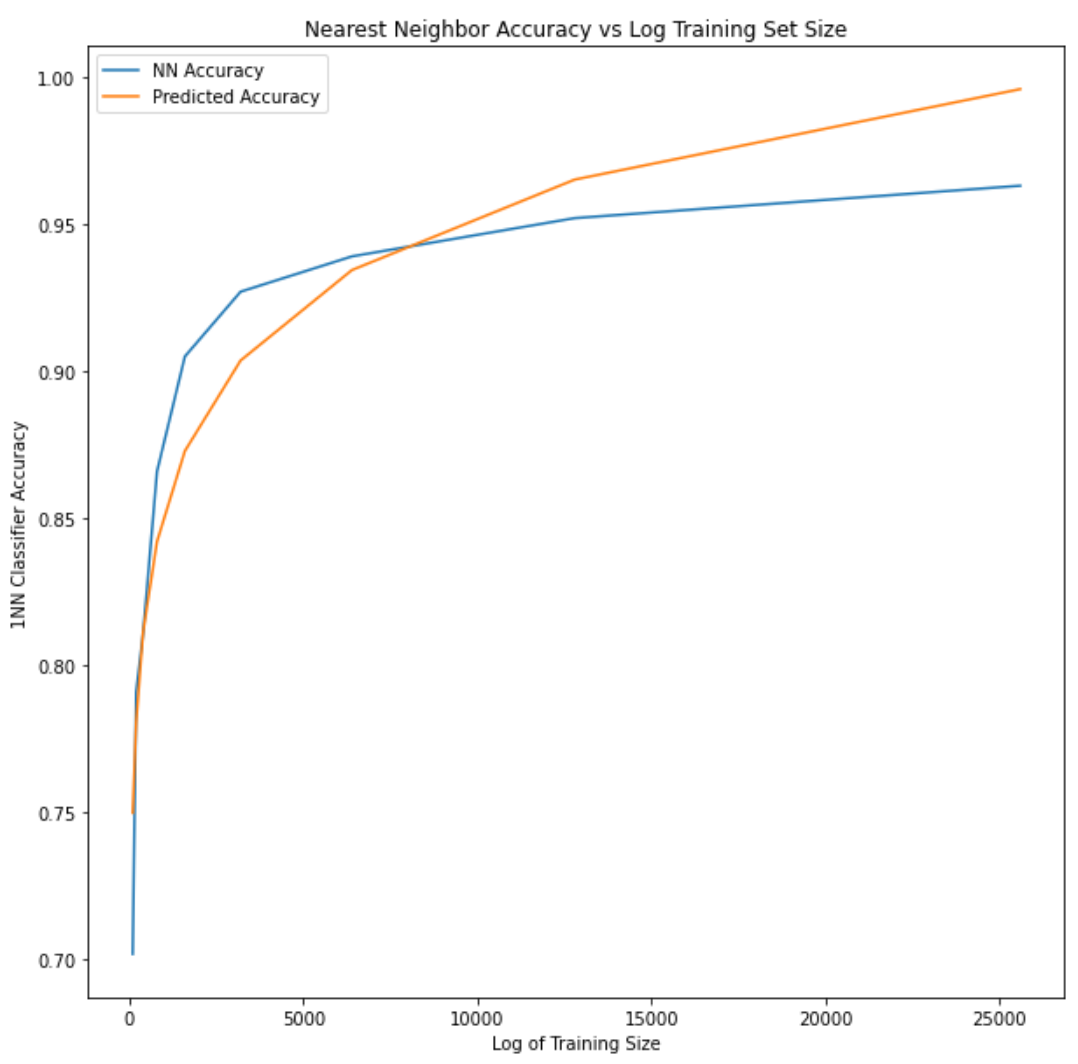
\includegraphics[width=7cm]{4.2.png}
    \end{center}
    
    As the left graph shows, using a linear regression is ill-suited to predict KNN accuracy, as KNN accuracy increases roughly logarithmically with the training set size, not linearly. The $R^2$ of the linear regression is a mere 0.4177. This can be improved somewhat by training the linear classifier on the log of the training size instead, shown on the right.
    
    While the graph on the right is still not a perfect fit, this greatly improves the prediction accuracy, with $R^2 = 0.9068$.
    
    The following table shows the predicted accuracy for certain large training sizes.
    
    \begin{tabular}{| c | c |}
    \hline
    \textbf{Training Set Size} & \textbf{Predicted Accuracy} \\
    \hline
    60,000 & 1.236 \\
    \hline
    120,000 & 1.637 \\
    \hline
    1,000,000 & 7.522 \\
    \hline
    \end{tabular}
    
    As this table shows, a linear regression model has nothing stopping it from predicting $>$ 100\% accuracy.

    
\newpage

\item % 5
    According to the confusion matrix (shown below), the most commonly confused digits are '4' and '9'. Some sample digits are also shown below.
    
    \begin{center}
    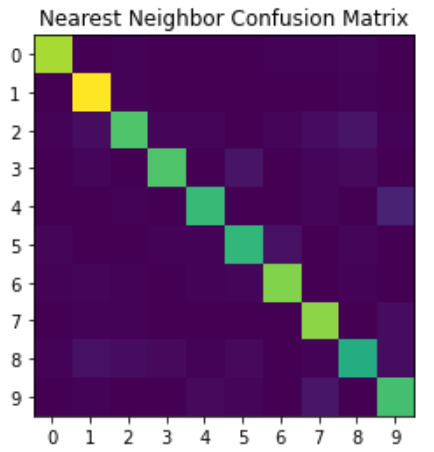
\includegraphics[width=5cm]{5.1.png}
    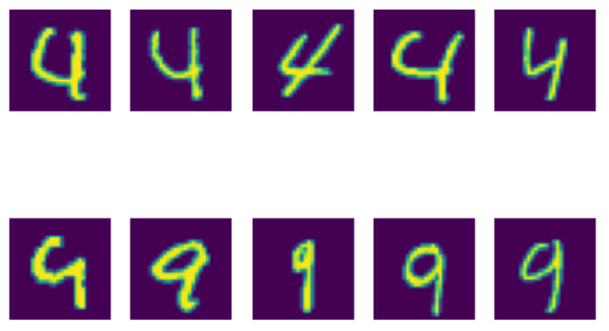
\includegraphics[width=9cm]{5.2.png}
    \end{center}

\item % 6
    For this, I found that the more ``confusing'' the training set, the more robust the classifier ended up being. With this in mind, I designed the blur matrix to make 4 and 9 as close to each other as possible, with stronger left-right bluring. This resulted in a classifier with 91.4\% accuracy on unblurred digits.
    
    The blur matrix I used is shown below, along with a sample before/after digit:
    
    \begin{tabular}{| c | c | c |}
    \hline
    1 & 1 & 3 \\
    \hline
    2 & 0 & 2 \\
    \hline
    3 & 1 & 1 \\
    \hline
    \end{tabular}
    
    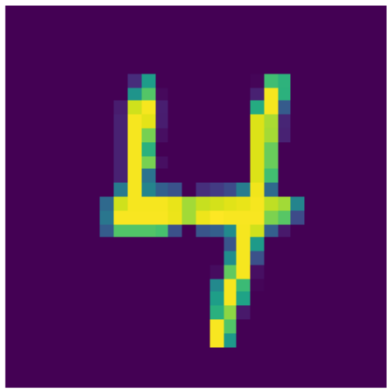
\includegraphics[width=2cm]{6.1.png}
    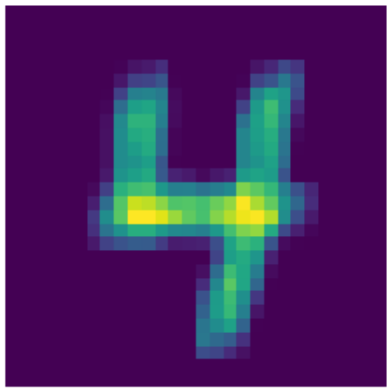
\includegraphics[width=2cm]{6.2.png}

    With this, I had the following performance characteristics:
    
    \begin{tabular}{| c | c | c |}
    \hline
    \textbf{Accuracy} & \textbf{Unblurred Dataset} & \textbf{Blurred Dataset} \\
    \hline
    \textbf{Unblurred Classifier} & 0.884 & 0.870 \\
    \hline
    \textbf{Blurred Classifier} & 0.914 & 0.907 \\
    \hline
    \end{tabular}

\item % 7
    The Bernoulli Naive Bayes accuracy was 0.814 \\
    The Multinomial Naive Bayes accuracy was 0.807
    
    Using multinomial NB did not improve the results, because the stroke intensity of the pen when drawing a digit does not normally factor in to how you should interpret it. When rendering a digit, ideally each pixel would only have one of two values: light or dark.
    
\item % 8
    When cross-validating, I found the best value for $\alpha$ to be 0.001. When $\alpha$ was too close to 0, the accuracy decreased, but still keeping $\alpha$ near 0 helped increase the accuracy of the classifier.
    
\item % 9
    With an untuned Gaussian Naive Bayes classifier, I had an accuracy of 0.593 \\
    By tuning the \texttt{var\_smoothing} hyperparameter to 0.06765, I improved its accuracy to 0.82
    
    By increasing this hyperparameter slightly, I made the classifier include neighboring data points when classifying images, acting similar to the Gaussian blur effect I applied earlier. This helped the Gaussian classifier perform similarly to the Bernoulli classifier.
    
\newpage

\item % 10
    First, I'll generate the ``ground truth'' probabilities, both raw and quantized.
    
    \begin{center}
    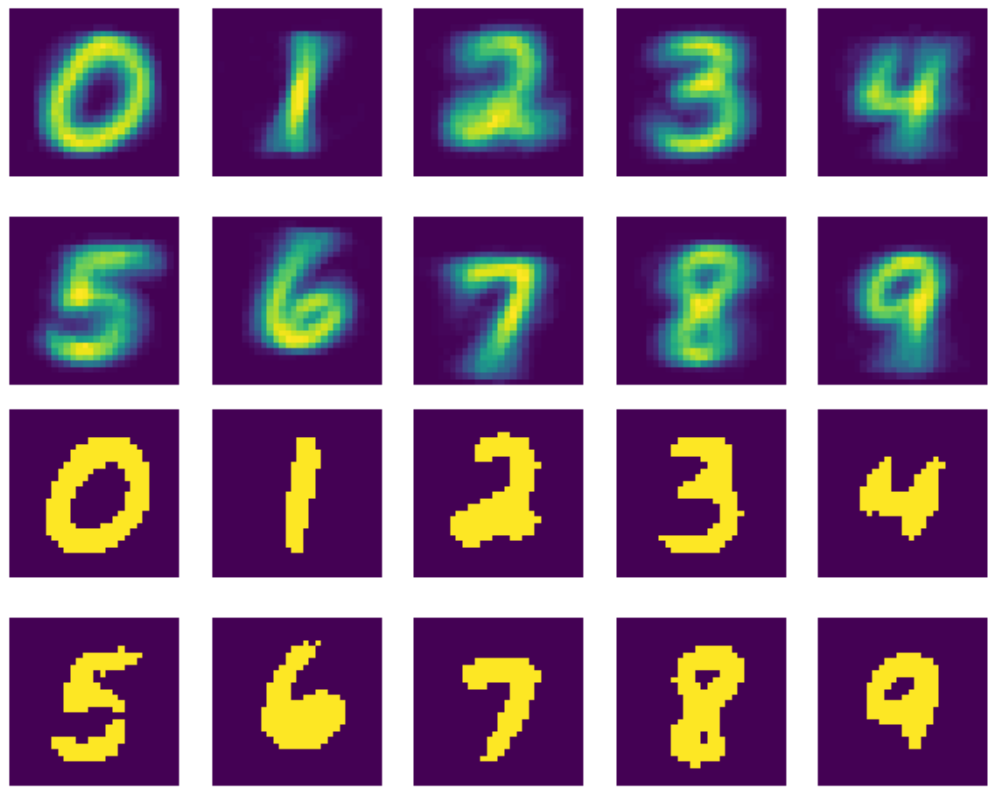
\includegraphics[width=9cm]{10.1.png}
    \end{center}
    
    Next, here are 20 samples of each digit, randomly setting pixels on or off. Note that the green/yellow coloring is just an artifact caused by not having enough space for 28 pixels per subplot.
    
    \begin{center}
    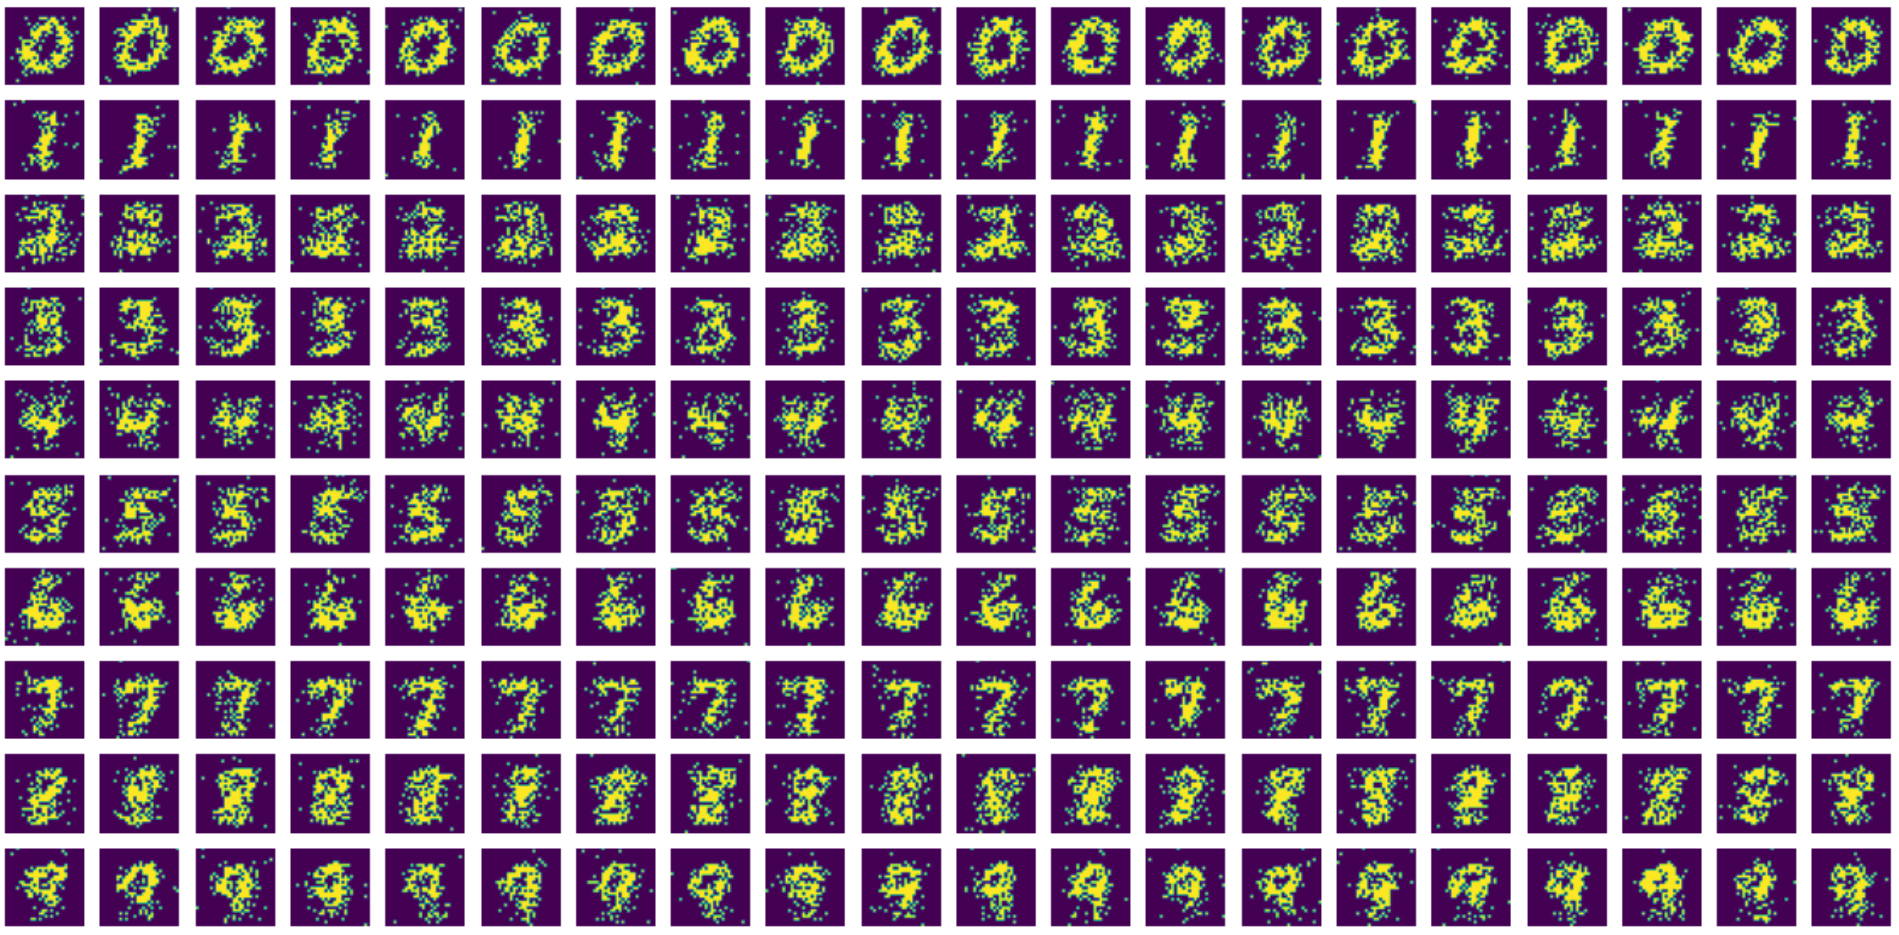
\includegraphics[width=\linewidth]{10.2.png}
    \end{center}
    
\item % 11
    With $\alpha = 0.001$, I found the following accuracies:
    
    \begin{Verbatim}
p(pred) 0.0000000000000 - 0.5000000000000   total =   0   accuracy = 0.000
p(pred) 0.5000000000000 - 0.9000000000000   total =  31   accuracy = 0.355
p(pred) 0.9000000000000 - 0.9990000000000   total =  67   accuracy = 0.433
p(pred) 0.9990000000000 - 0.9999900000000   total =  59   accuracy = 0.458
p(pred) 0.9999900000000 - 0.9999999000000   total =  46   accuracy = 0.652
p(pred) 0.9999999000000 - 0.9999999990000   total =  62   accuracy = 0.774
p(pred) 0.9999999990000 - 0.9999999999900   total =  33   accuracy = 0.788
p(pred) 0.9999999999900 - 0.9999999999999   total =  43   accuracy = 0.791
p(pred) 0.9999999999999 - 1.0000000000000   total = 659   accuracy = 0.938
    \end{Verbatim}

    Based on this performance, I would describe this as a weakly calibrated classifier.

\end{enumerate}

\end{document}
